% meta.concepts: resultant, 2D 
% meta.tags: realistic
% acknowledge: Organic Navigation photos
% inspiration: Beer, Johnston, and Mazurek (Problem 2.9, 12th Edition)

A skid-steer loader breaks down at a job site.  Two tow ropes are attached pulling along $AB$ and $AC$.  The tension in rope $AB$ is $3 kN$.  The goal is to pull along $AC$ such that a $4.8-kN$ force is applied horizontally at point $A$, thereby pulling the skid-steer loader safely away from the job site.

Determine the tension and direction ($\alpha$) required to pull along $AC$ to achieve this.

\begin{figure}[ht!]
  \centering
  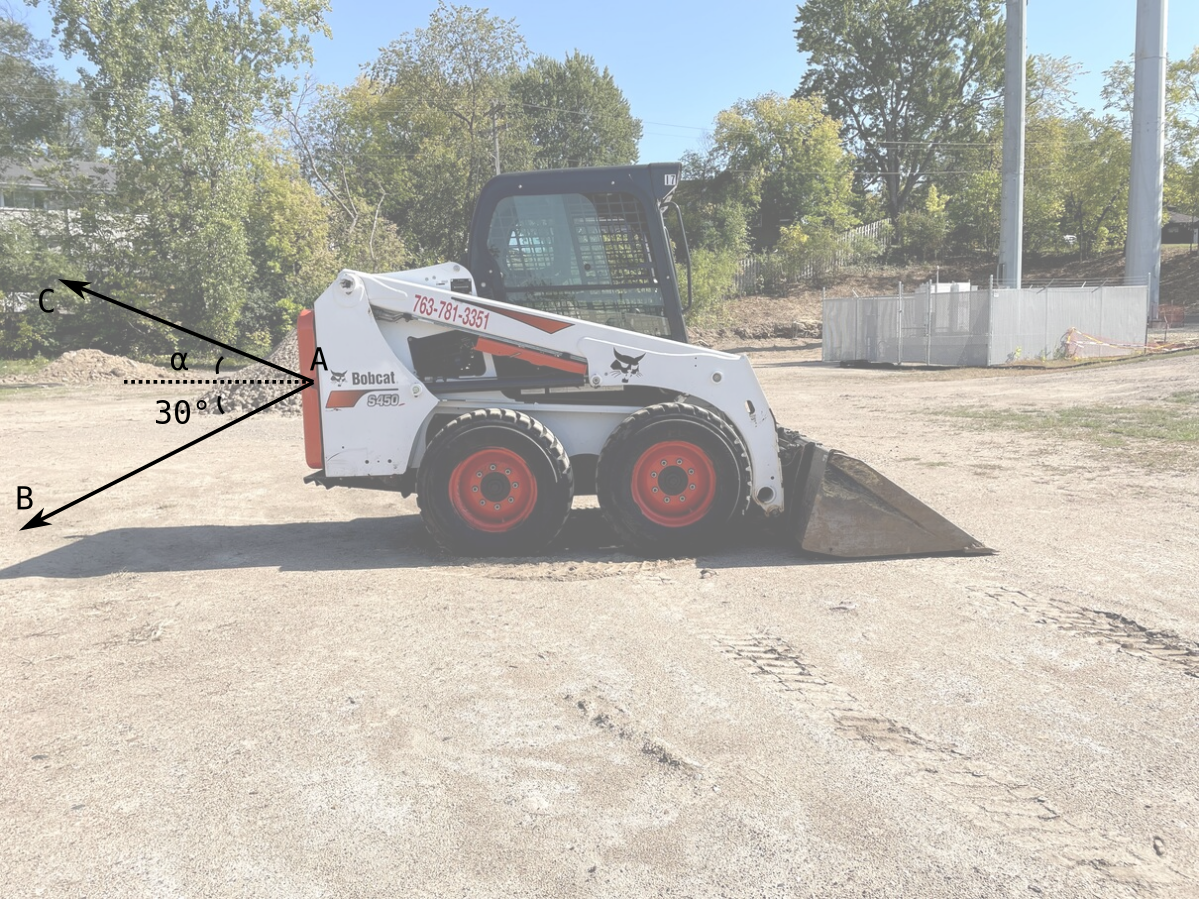
\includegraphics[width=5.0in]{fig.png}
\end{figure}

